\section{Analysis Results}
\label{sec:hh_results}

As with the analysis presented in Chapter~\ref{chap:search_stop}, a profile likelihood
fit is performed, including all CRs and SRs of the analysis and with the observed
data in all regions used as a constraint.
The result of running this fit is shown in Table~\ref{tab:hh_final_sr_yields}.
The observed data and post-fit MC prediction agrees quite well in SR-SF.
In SR-DF there is a slight excess observed in the data relative to the MC prediction.
This excess in SR-DF is not statistically significant however, and amounts to only a $1.05\sigma$ excess
(null $p_0$-value of 0.15).
Figures~\ref{fig:hh_sr_kin_0}-\ref{fig:hh_sr_kin_3} present kinematic distributions comparing
the observed data and post-fit MC prediction for the SM backgrounds in the SR selections.
Figures~\ref{fig:hh_sr_kin_1} and \ref{fig:hh_sr_kin_2} show the \dhh distributions in detail
in SR-DF and SR-SF, respectively.

As there is no significant deviation between the prediction and observed data,
indicating that there is no evidence for enhanced production of Higgs boson pairs, 95\% CL
cross-section upper-limits are derived for the SM-like non-resonant Higgs boson pair
production.
These results are reported in Table~\ref{tab:hh_bbww_xsec_ul} and are with respect to the
$pp \rightarrow hh$ production process, having taken into account the branching ratio for the dilepton $hh \rightarrow \bbww$
decay.
That is, the 95\% CL UL reported in Table~\ref{tab:hh_bbww_xsec_ul} are on \sigmaHH, and not
on $\sigmaHH \times \text{BR}(hh \rightarrow \bbww) \times \text{BR}(WW^* \rightarrow \ell \nu \ell \nu)$.
The effect of the $1.05\sigma$ excess in SR-DF is seen in the observed 95\% CL UL, which in Table~\ref{tab:hh_bbww_xsec_ul}
is seen to be larger than the expected value by roughly $1\sigma$.
Figure~\ref{fig:hh_ul_comp} illustrates the results listed in Table~\ref{tab:hh_bbww_xsec_ul},
while also comparing them to the leading $hh$ searches (c.f. Figure~\ref{fig:hh_comb_36}): $hh \rightarrow \bbbb$,
$hh \rightarrow \bbtautau$, and $hh \rightarrow \bbyy$.
The comparisons with the other analyses are made only with respect to the expected 95\% CL cross-section upper-limits.
It should be remembered that the other analyses in Figure~\ref{fig:hh_comb_36} are based only on the partial Run 2
dataset, collected in 2015--2016 and comprised of $36.2$\,fb$^{-1}$ of $pp$ collision data.
However, the analysis presented in this chapter is the first time that this search has been performed
in ATLAS and it is already improving the prospects of searches for $hh$ in the \bbww channel by roughly
a factor of 10 (c.f. Figure~\ref{fig:hh_comb_36}).
At the time of writing, work is already started on improving the results presented here.
One such improvement, based on performing a multi-binned shape analysis wherein the full \textit{shape} of the \dhh
distribution is used as input to the hypothesis tests --- as opposed to simply \textit{cutting} on the \dhh distribution
and defining simple signal regions as in Table~\ref{tab:hh_sr_def} --- is expected to increase the sensitivity to the $hh \rightarrow \bbww$ signal process
substantially.



\begin{table}[!htb]
    \begin{center}
        \caption{
            Observed and predicted yields in the SRs for the dilepton $hh \rightarrow \bbww$ search.
        }
        \label{tab:hh_final_sr_yields}
        \begin{tabular}{l | c c}
        \hline
        \hline
                & \multicolumn{2}{c}{\textbf{Regions}} \\
            \cline{2-3}
            \textbf{Process} & \textbf{SR-SF} & \textbf{SR-DF} \\
            \hline
            Observed Data   & 16 & 9 \\
            \hline
            Post-fit Total SM & $14.88 \pm 2.12$ & $4.88 \pm 1.24$ \\
            \hline
            Post-fit \ttbar & $2.57 \pm 0.97$ & $1.74 \pm 0.66$ \\
            Post-fit Single-top $Wt$ & $2.27 \pm 0.54$ & $2.04 \pm 0.64$ \\
            Post-fit $Z$+heavy-flavor & $7.76 \pm 1.04$ & $0.21 \pm 0.05$ \\
            \hline
            SM & $14.12 \pm 2.05$ & $5.83 \pm 1.42$ \\
            \hline
            \ttbar & $3.26 \pm 1.17$ & $2.20 \pm 0.80$ \\
            Single-top $Wt$ & $2.88 \pm 0.59$ & $2.58 \pm 0.75$ \\
            $\ttbar + V$ & $0.59 \pm 0.07$ & $0.07  \pm 0.06$ \\
            $Z$+heavy-flavor & $5.71 \pm 0.74$ & $0.15 \pm 0.04$ \\
            $Z$+light-flavor & $0.32 \pm 0.14$ & $0.00 \pm 0.00$ \\
            Single-higgs & $0.72 \pm 0.09$ & $0.32 \pm 0.06$ \\
            Fakes & $0.54 \pm 0.38$ & $0.42 \pm 0.36$ \\
        \hline
        \hline
        \end{tabular}
    \end{center}
\end{table}

\begin{table}[!htb]
    \begin{center}
        \caption{
            Expected and observed 95\% CL upper-limits on the Standard Model, non-resonant $hh$
            production cross-section ($\sigma(pp \rightarrow hh)$) and on
            the ratio of the upper-limit on this value to the value predicted in the SM
            ($\sigmaSM = 31.05$ fb).
            The observed limits are in the right most column.
            The $\pm 1 \sigma$ and $\pm 2\sigma$ excursions from the median expected value incorporate the
            effects of the analysis' systematic uncertainties.
        }
        \label{tab:hh_bbww_xsec_ul}
        \begin{tabular}{l | c | c | c | c | c || c }
            \hline
            \hline
                    & $-2\sigma$ & $-1 \sigma$ & \textbf{Median Expected} & $+1 \sigma$ & $+2 \sigma$ & \textbf{Observed} \\
            \hline
                95\% CL UL $\sigma (pp \rightarrow hh)$ [pb] & $0.465$ & $0.641$ & $0.920$ & $1.363$ & $1.990$ & $1.290$ \\
                \sigmaRatio & $14.97$ & $20.66$ & $29.63$ & $43.89$ & $64.02$ & $41.54$ \\
            \hline
            \hline
        \end{tabular}
    \end{center}
\end{table}

%%%%%%%%%%%%%%%%%%%%%%%%%%%%%%%%%%%%%%%%%%%%%%%%%%%%%%%%%%%%%%%%%%%%%%%%%%%%%%%%%%%%%%%%%%%%
%%%%%%%%%%%%%%%%%%%%%%%%%%%%%%%%%%%%%%%%%%%%%%%%%%%%%%%%%%%%%%%%%%%%%%%%%%%%%%%%%%%%%%%%%%%%
%%%%%%%%%%%%%%%%%%%%%%%%%%%%%%%%%%%%%%%%%%%%%%%%%%%%%%%%%%%%%%%%%%%%%%%%%%%%%%%%%%%%%%%%%%%%
%
% SR KIN PLOTS
%
%%%%%%%%%%%%%%%%%%%%%%%%%%%%%%%%%%%%%%%%%%%%%%%%%%%%%%%%%%%%%%%%%%%%%%%%%%%%%%%%%%%%%%%%%%%%
%%%%%%%%%%%%%%%%%%%%%%%%%%%%%%%%%%%%%%%%%%%%%%%%%%%%%%%%%%%%%%%%%%%%%%%%%%%%%%%%%%%%%%%%%%%%
%%%%%%%%%%%%%%%%%%%%%%%%%%%%%%%%%%%%%%%%%%%%%%%%%%%%%%%%%%%%%%%%%%%%%%%%%%%%%%%%%%%%%%%%%%%%

\begin{figure}[!htb]
    \begin{center}
        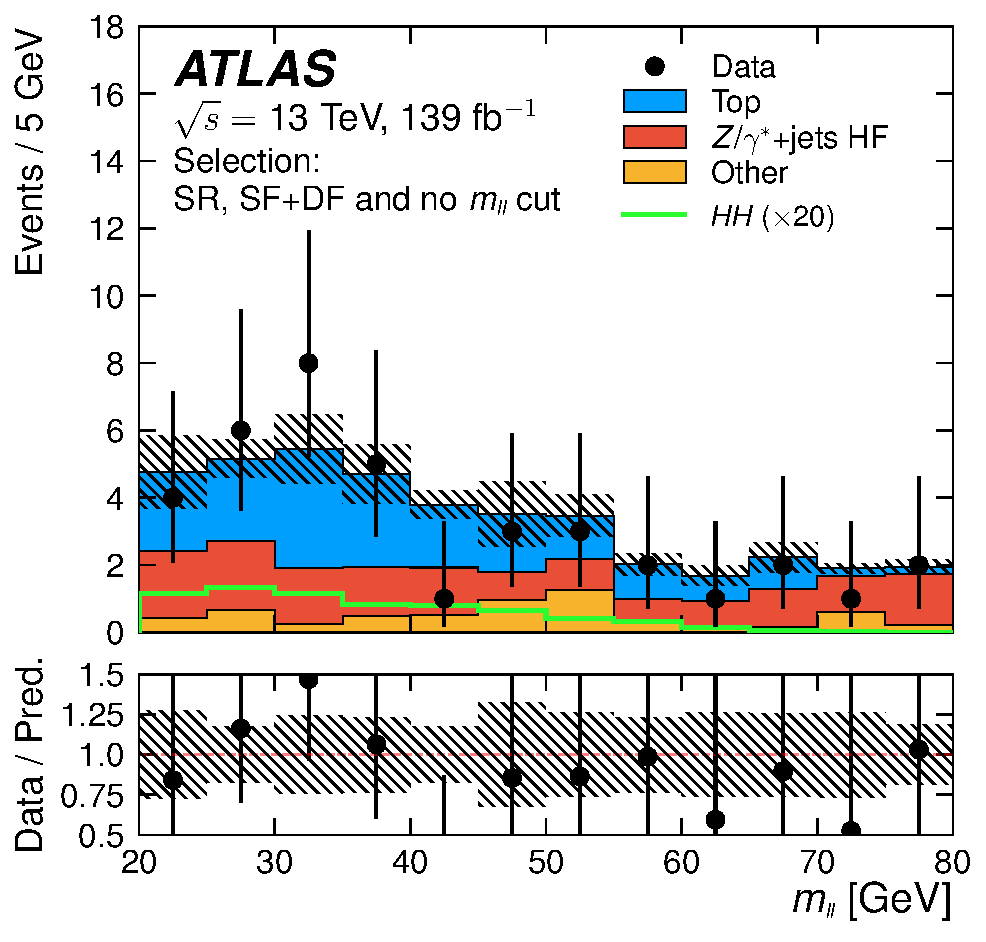
\includegraphics[width=0.48\textwidth]{figures/search_hh/results/sr_plots/srIncNoMllDhh_mll}
        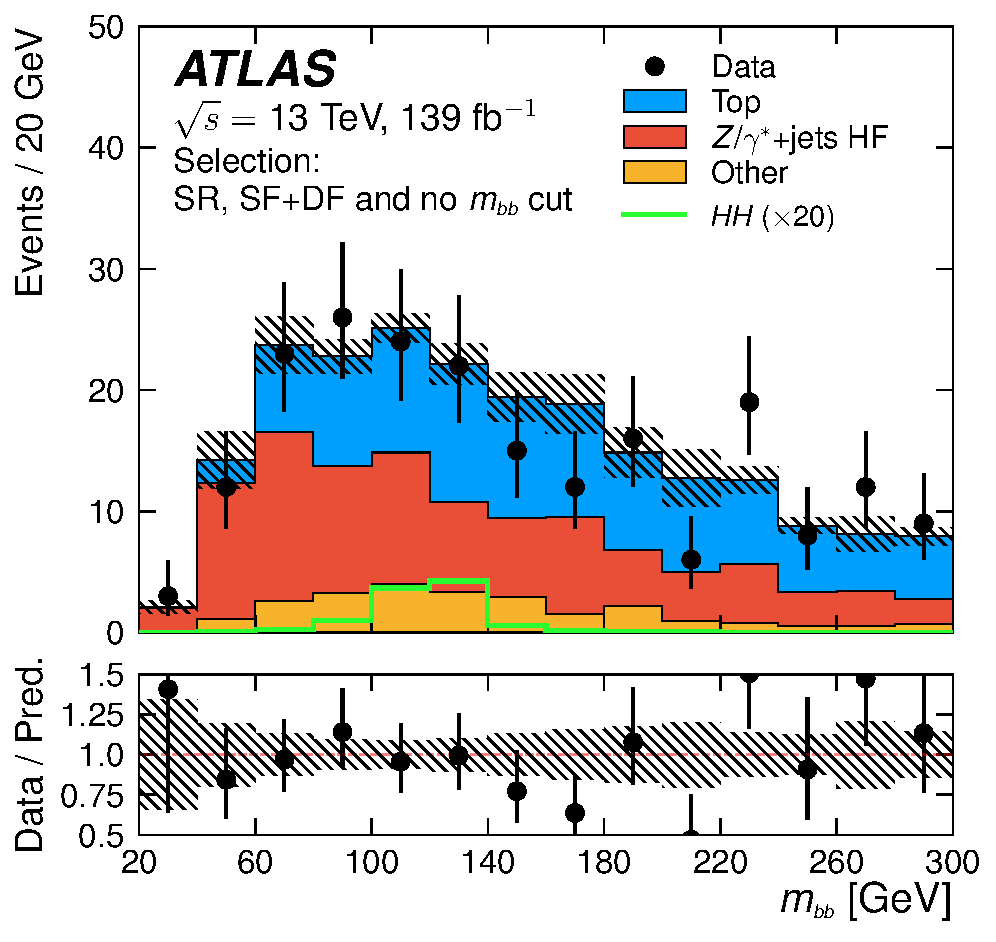
\includegraphics[width=0.48\textwidth]{figures/search_hh/results/sr_plots/srIncNoMbbDhh_mbb}
        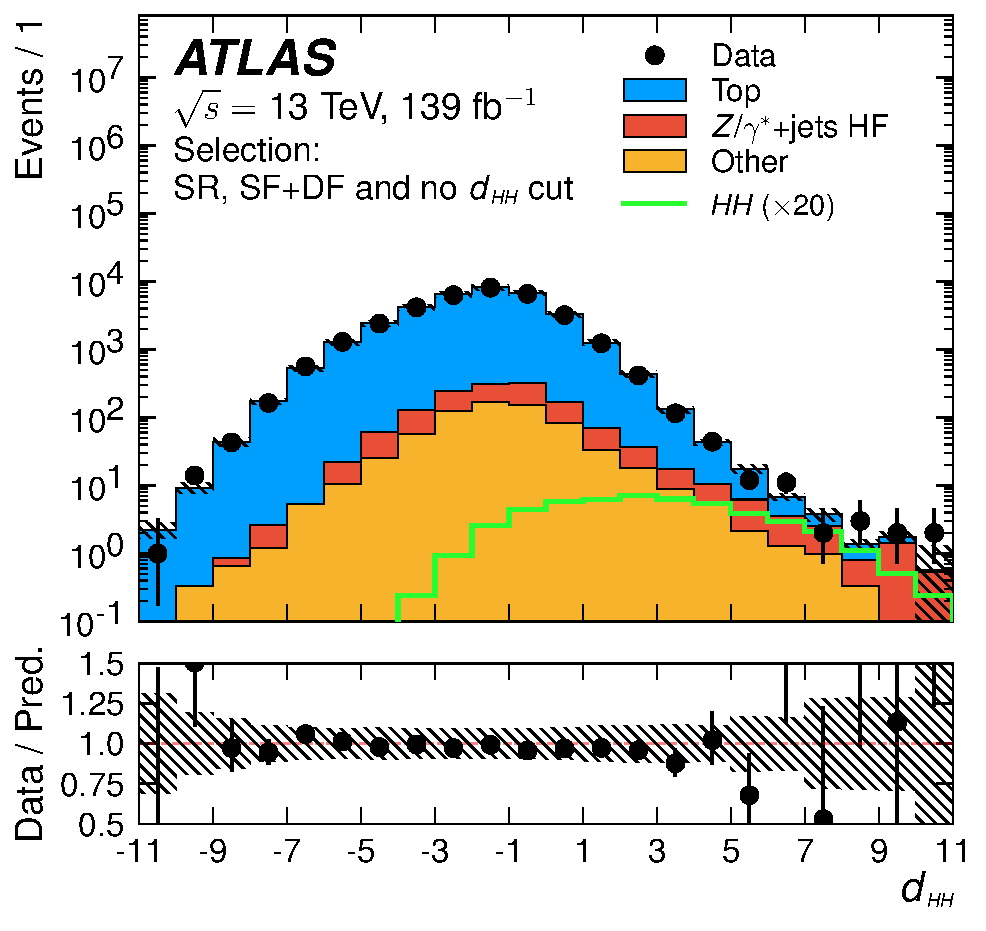
\includegraphics[width=0.48\textwidth]{figures/search_hh/results/sr_plots/srIncNoDhh_NN_d_hh}
        \caption{
            Distributions of $m_{\ell \ell}$ (\textit{\textbf{left}}), $m_{bb}$ (\textit{\textbf{right}}),
            and \dhh (\textit{\textbf{bottom}}).
            The distributions are shown after the fit to data in the control regions under the background-only hypothesis.
            Each distribution includes both the SF and DF events and imposes the analysis SR requirements
            on all quantities except for the one being plotted.
            The SR requirement on \dhh in the $m_{\ell\ell}$ and $m_{bb}$ distributions is relaxed to $\dhh > 5$.
            The dilepton $hh \rightarrow \bbww$ signal, labeled as `$HH$', is shown with its cross-section scaled
            by a factor of 20 relative to the SM prediction for visualization purposes.
            The ratio of the data to the sum of the backgrounds is shown in the lower panel of each figure.
            The hatched bands indicate the combined statistical and systematic uncertainty.
        }
        \label{fig:hh_sr_kin_0}
    \end{center}
\end{figure}

\begin{figure}[!htb]
    \begin{center}
        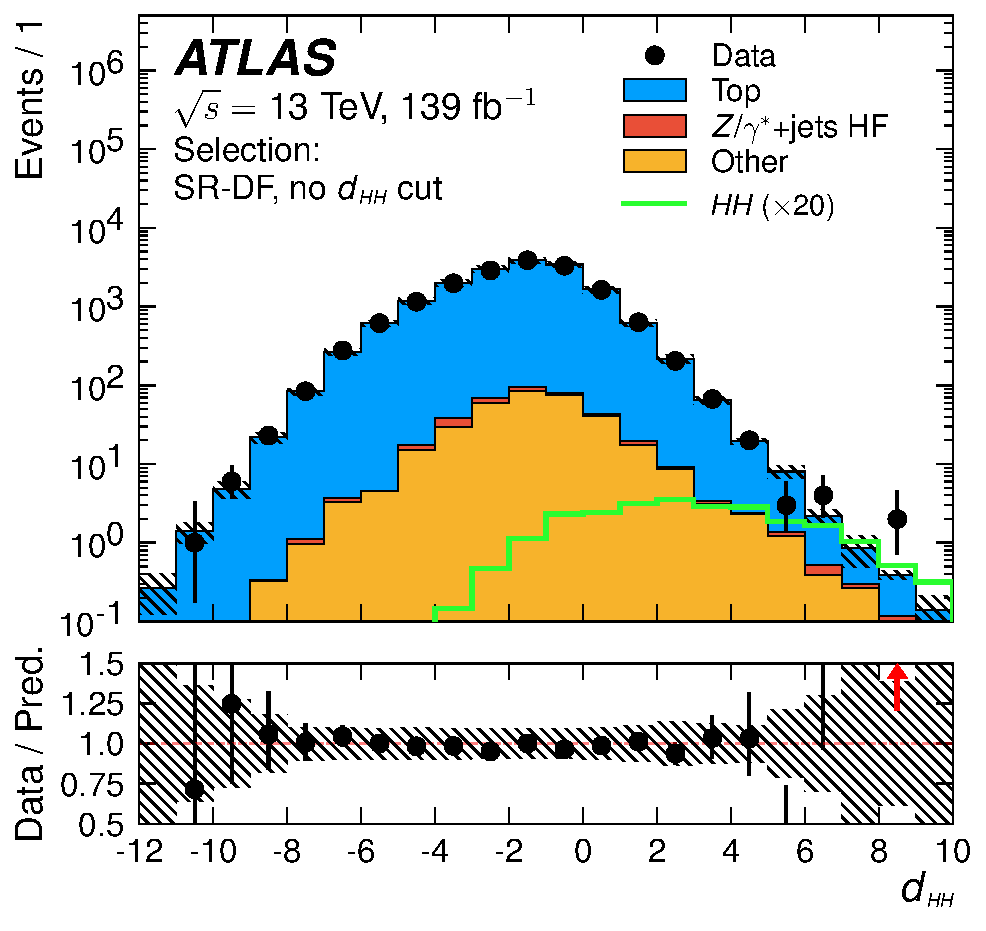
\includegraphics[width=0.48\textwidth]{figures/search_hh/results/sr_plots/srDFNoDhh_NN_d_hh}
        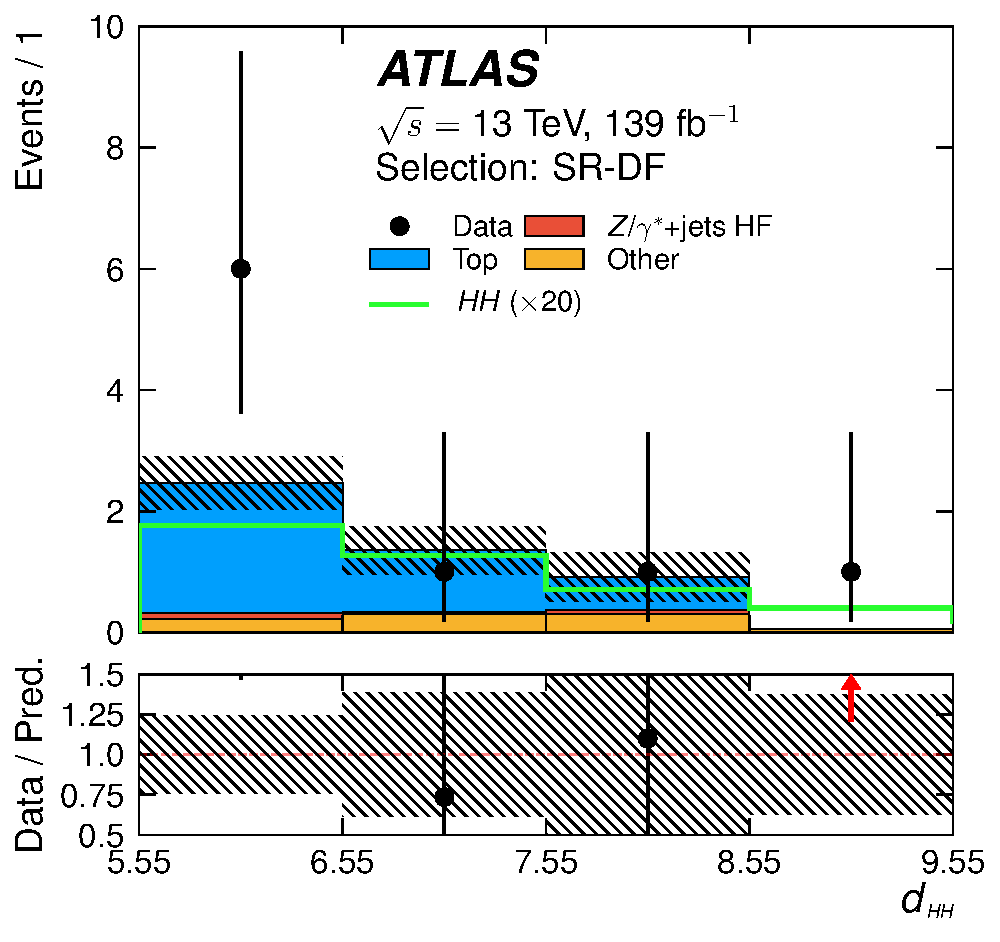
\includegraphics[width=0.48\textwidth]{figures/search_hh/results/sr_plots/srDFNoDhhCloseCut_NN_d_hh}
        \caption{
            Distributions of the \dhh observable in SR-DF without the \dhh selection applied (\textit{\textbf{left}})
            and with the \dhh selection ($\dhh > 5.55$) applied (\textit{\textbf{right}}).
            The dilepton $hh \rightarrow \bbww$ signal, labeled as `$HH$', is shown with its cross-section scaled
            by a factor of 20 relative to the SM prediction for visualization purposes.
            The ratio of the data to the sum of the backgrounds is shown in the lower panel of each figure.
            The hatched bands indicate the combined statistical and systematic uncertainty.
        }
        \label{fig:hh_sr_kin_1}
    \end{center}
\end{figure}
\begin{figure}[!htb]
    \begin{center}
        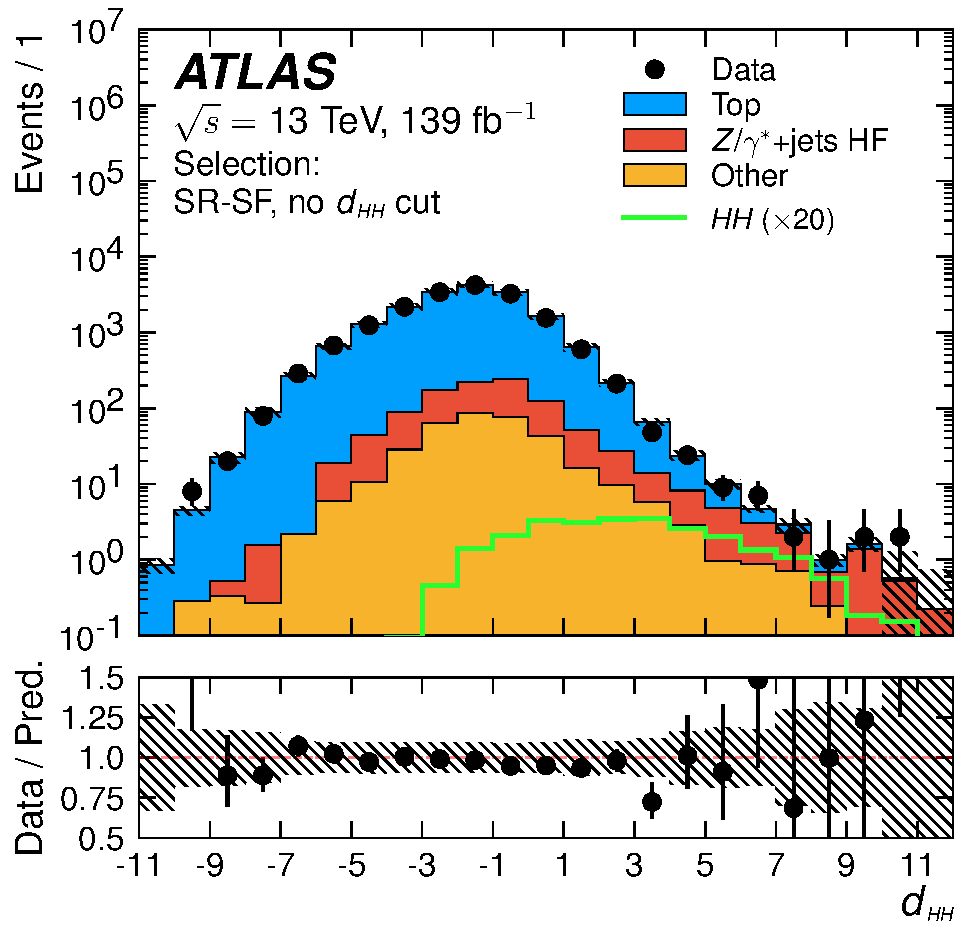
\includegraphics[width=0.48\textwidth]{figures/search_hh/results/sr_plots/srSFNoDhh_NN_d_hh}
        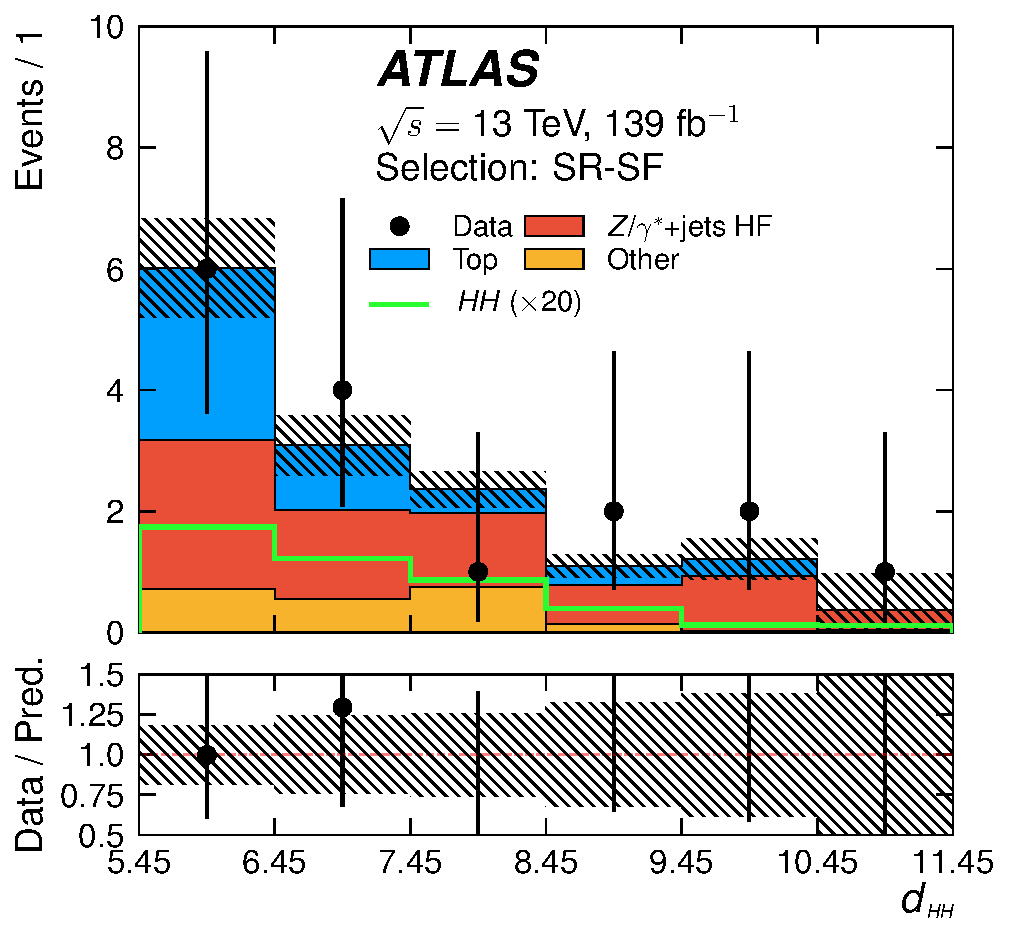
\includegraphics[width=0.48\textwidth]{figures/search_hh/results/sr_plots/srSFNoDhhCloseCut_NN_d_hh}
        \caption{
            Distributions of the \dhh observable in SR-SF without the \dhh selection applied (\textit{\textbf{left}})
            and with the \dhh selection ($\dhh > 5.45$) applied (\textit{\textbf{right}}).
            The dilepton $hh \rightarrow \bbww$ signal, labeled as `$HH$', is shown with its cross-section scaled
            by a factor of 20 relative to the SM prediction for visualization purposes.
            The ratio of the data to the sum of the backgrounds is shown in the lower panel of each figure.
            The hatched bands indicate the combined statistical and systematic uncertainty.
        }
        \label{fig:hh_sr_kin_2}
    \end{center}
\end{figure}

\begin{figure}[!htb]
    \begin{center}
        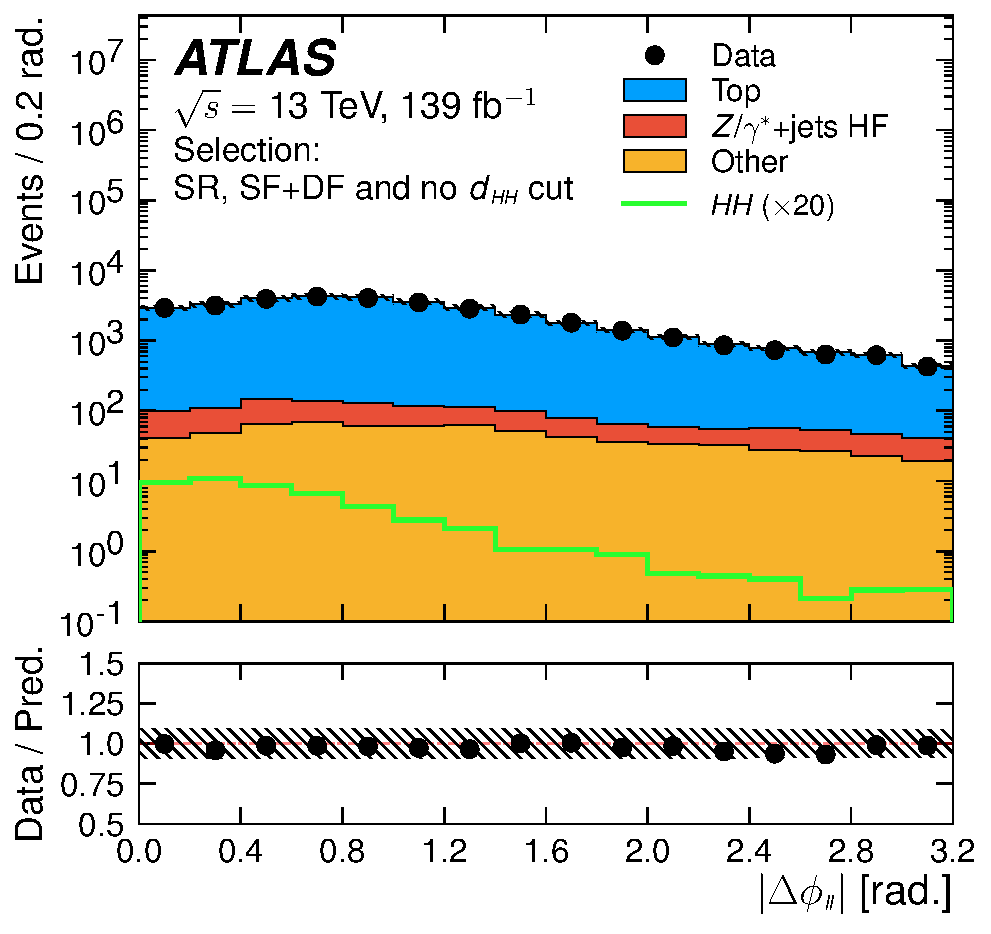
\includegraphics[width=0.48\textwidth]{figures/search_hh/results/sr_plots/srIncNoDhh_dphi_ll}
        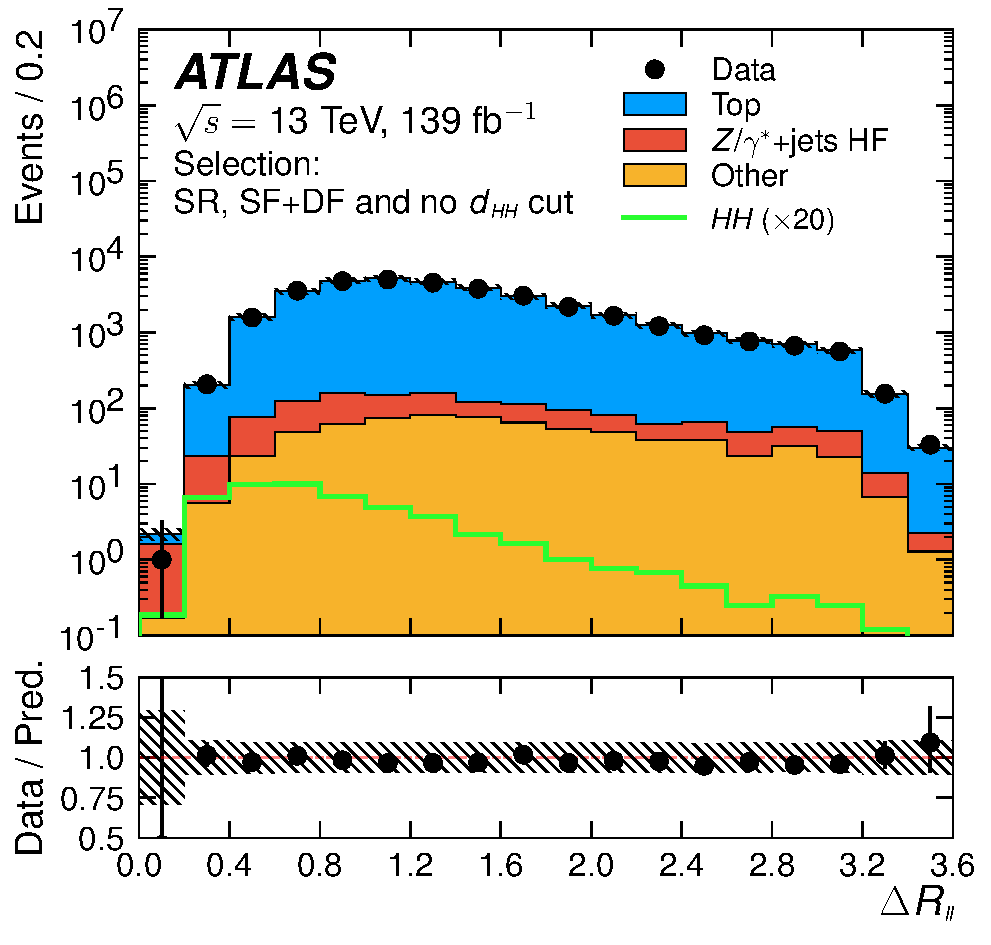
\includegraphics[width=0.48\textwidth]{figures/search_hh/results/sr_plots/srIncNoDhh_dRll}
        \caption{
            Distributions of the $|\dphill|$ and $\drll$ quantities in the analysis' SR selections,
            inclusive of SF and DF dilepton flavors and without the \dhh requirements.
            The dilepton $hh \rightarrow \bbww$ signal, labeled as `$HH$', is shown with its cross-section scaled
            by a factor of 20 relative to the SM prediction for visualization purposes.
            The ratio of the data to the sum of the backgrounds is shown in the lower panel of each figure.
            The hatched bands indicate the combined statistical and systematic uncertainty.
        }
        \label{fig:hh_sr_kin_3}
    \end{center}
\end{figure}

\begin{figure}[!htb]
    \begin{center}
        %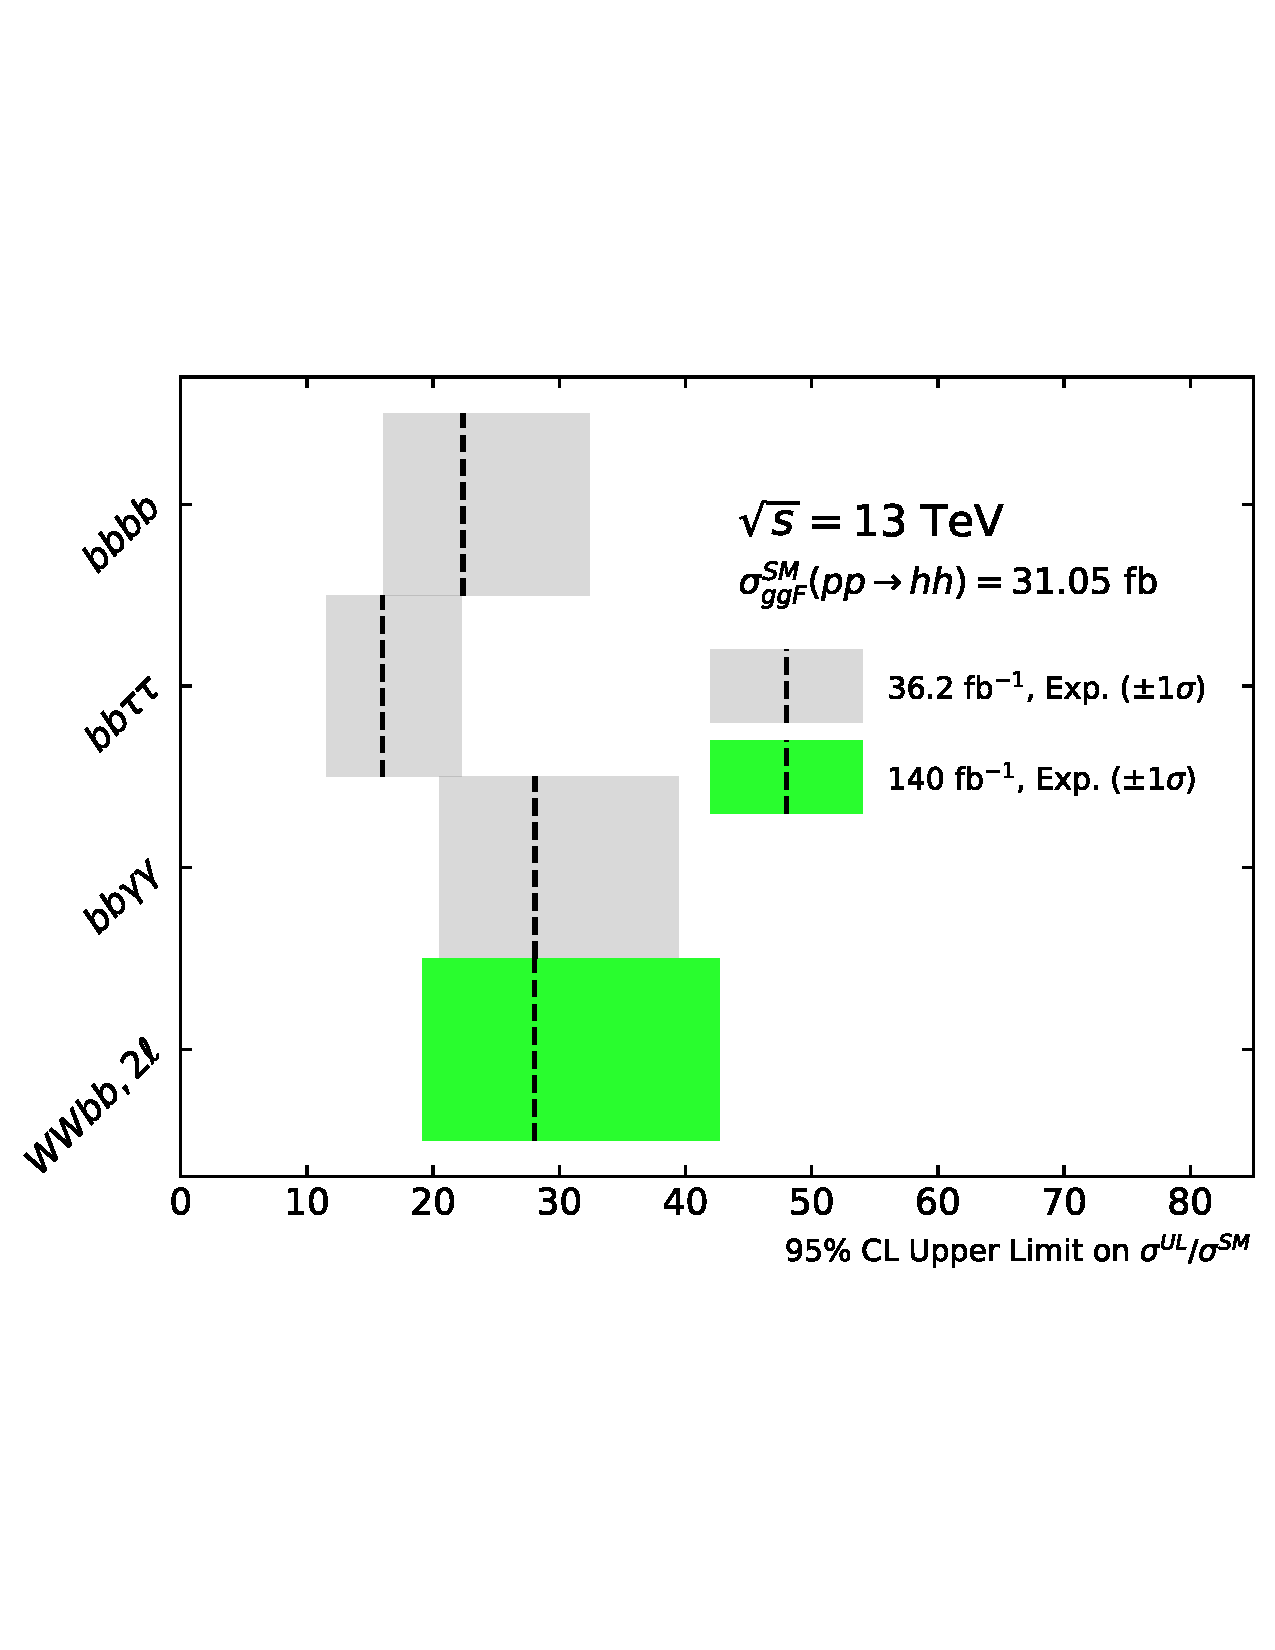
\includegraphics[width=0.75\textwidth]{figures/search_hh/results/atlas_jam_ul_plot_apr16}
        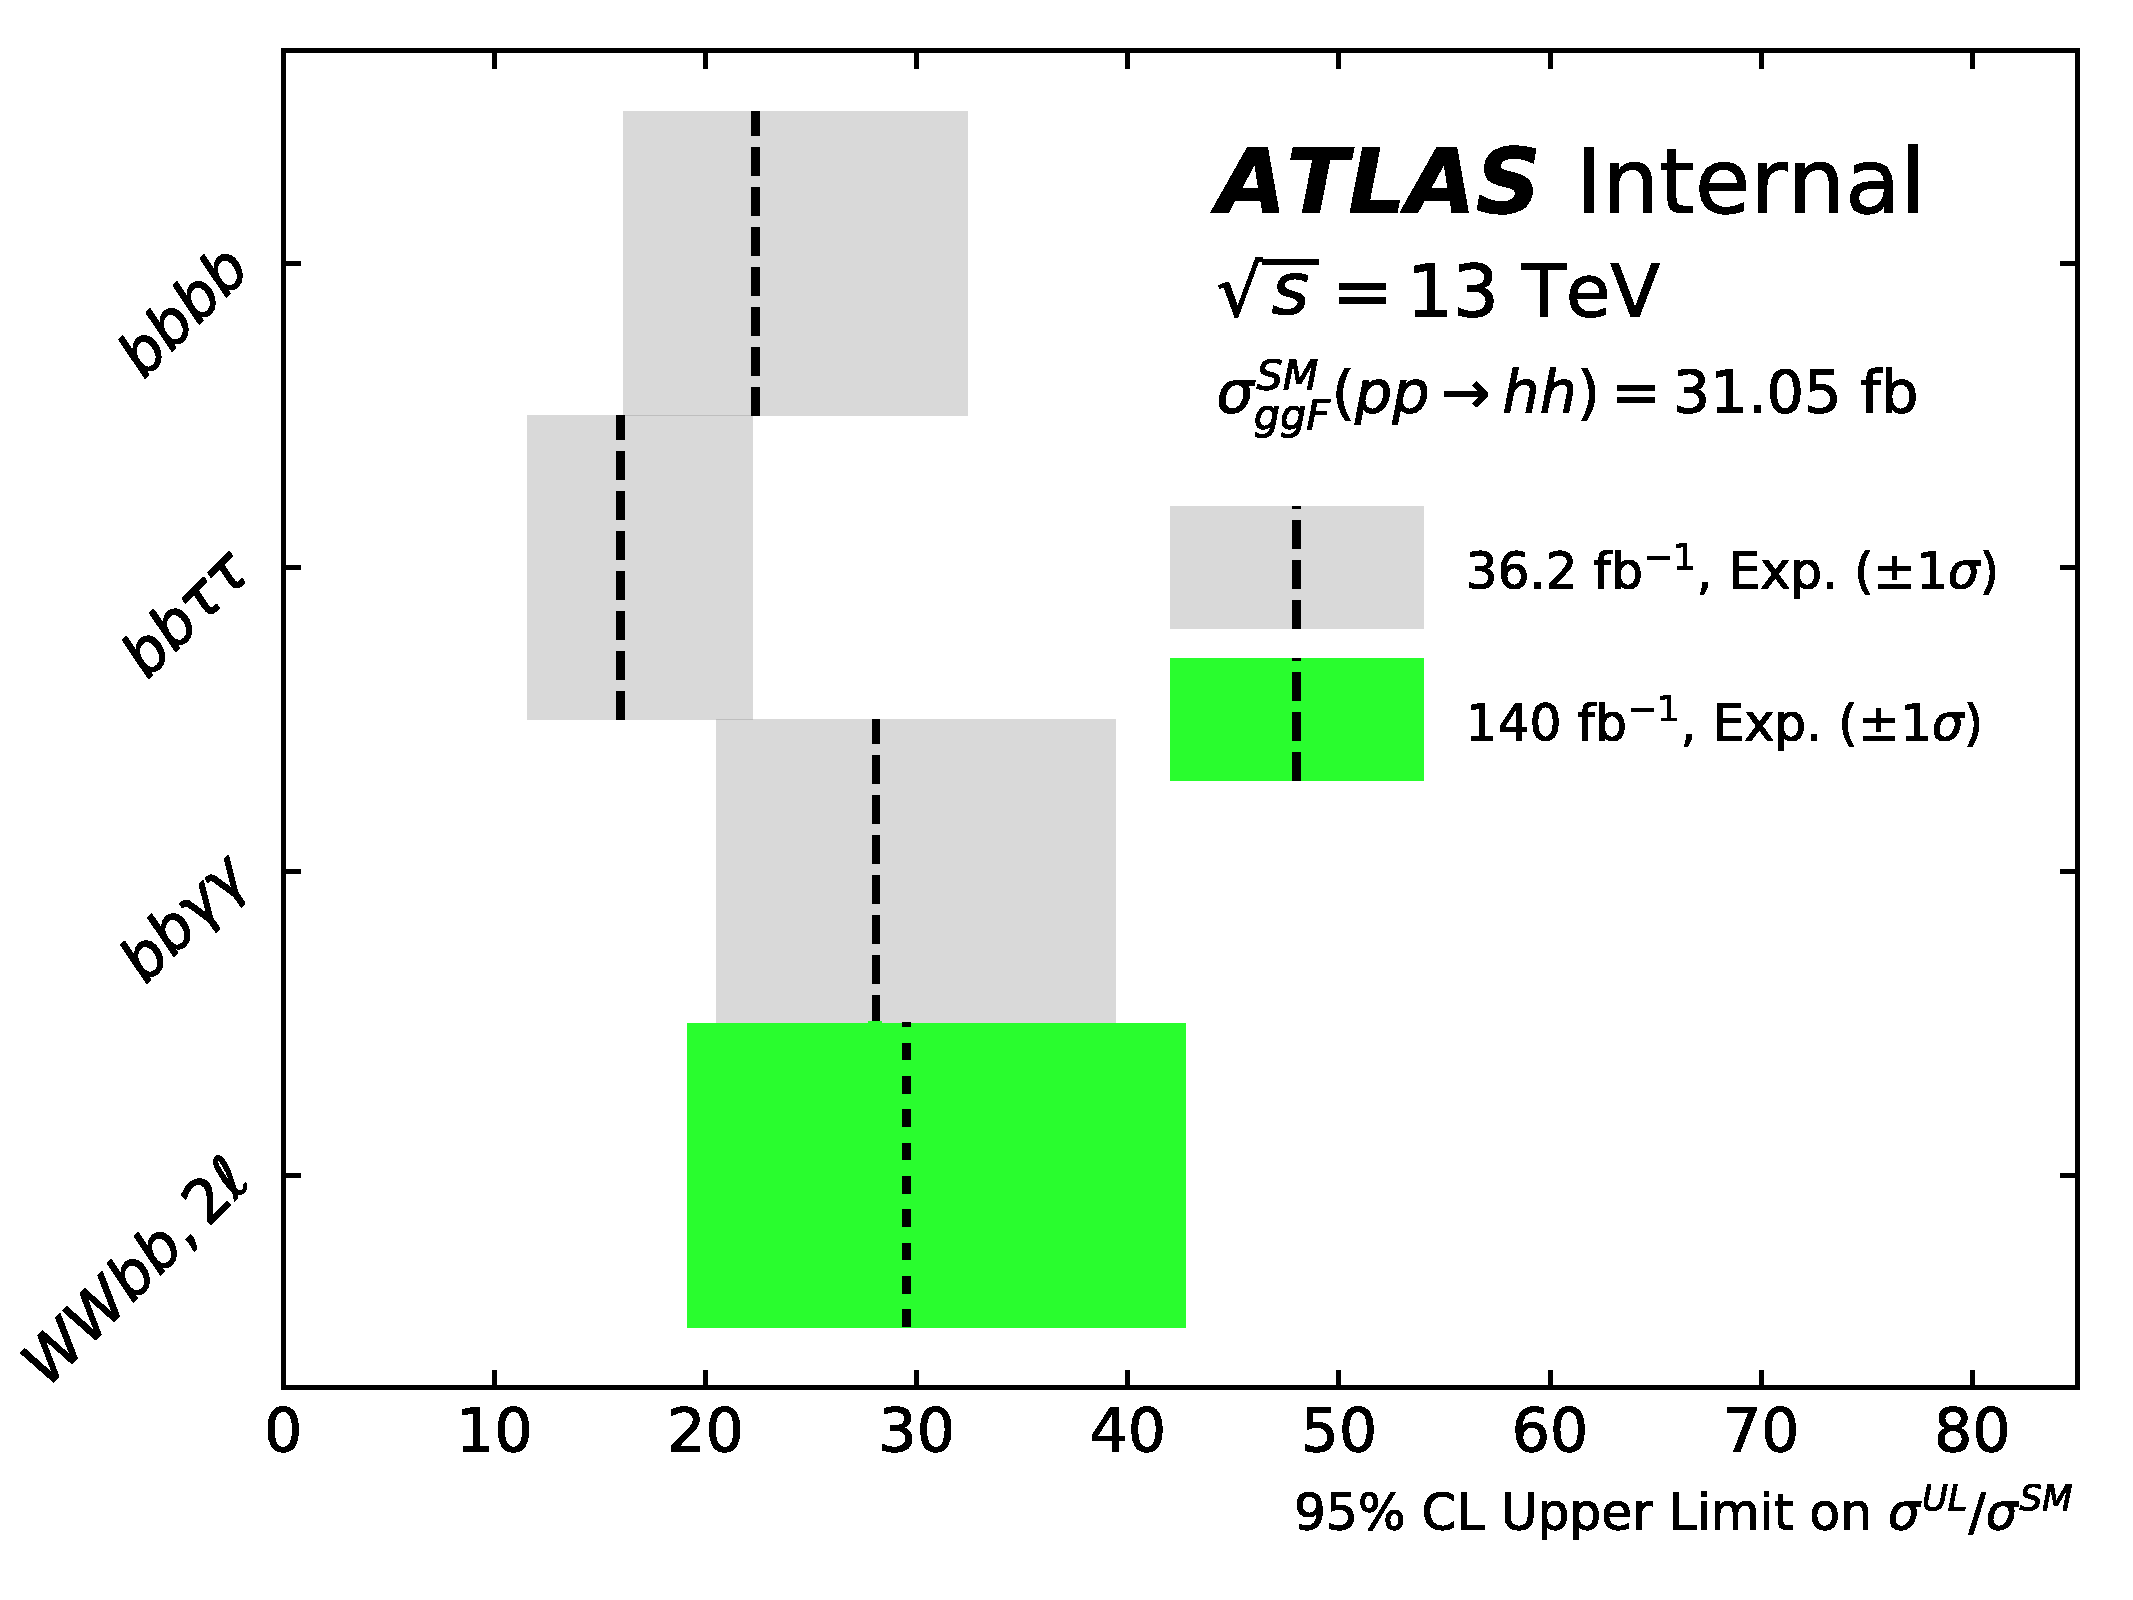
\includegraphics[width=0.6\textwidth]{figures/search_hh/results/hh_ul_compPDF}
        \caption{
            Summary plot showing the $hh$ production cross-section upper limit results, normalized to
            the SM prediction of 31.05\,fb, for the analysis presented in this thesis in green,
            based on the full Run 2 dataset of 139\,fb$^{-1}$ of $pp$ collision data.
            In grey, the partial Run 2 results based on 36\,fb$^{-1}$ of data are shown for comparison.
            Only the expected upper limits are shown.
        }
        \label{fig:hh_ul_comp}
    \end{center}
\end{figure}

In addition to the 95\% CL cross-section UL reported in Table~\ref{tab:hh_bbww_xsec_ul}, we also perform
a scan over the Higgs self-coupling parameter employed in the dilepton $hh \rightarrow \bbww$ signal MC sample
so that we may re-run the analysis for various non-SM hypotheses for the value of the Higgs self-coupling parameter,~$\lambda$.
The variations in the Higgs self-coupling are parametrized by $\kappa_{\lambda} = \lambda / \lambda_{SM}$, and this
value is scanned across the values $\kappa_{\lambda} \in [-20, 20]$.
Changing the value of $\kappa_{\lambda}$ changes the relative strength of the competing triangle
and box diagrams that lead to $hh$ production at LO at the LHC, with only the former sensitive to
the Higgs self-coupling parameter (c.f. Figure~\ref{fig:hh_feynman}).
Variations in $\kappa_{\lambda}$ can lead to either the box diagram or the triangle diagram being the dominant source of Higgs boson pairs.
%The signal kinematics can therefore change significantly as a result of variations in $\kappa_{\lambda}$.
Given the presence of the massive top-quarks, the Higgs bosons from the box diagram tend to have a harder transverse momenta
as compared to those from the triangle diagram, for example.
The Higgs bosons from predominantly box diagram production scenarios, then, lead to harder visible final state objects.
Further discussion about the effects of varying $\kappa_{\lambda}$ on the Higgs bosons' kinematics can
be found in Ref.~\cite{HHComb36}.

It should be stressed then, that the present analysis is in no way optimized for non-SM values of $\kappa_{\lambda}$.
For each new value of this parameter we simply perform the hypothesis tests using the same
sets of SRs and CRs described in the sections above.
The result of this $\kappa_{\lambda}$ scan are shown in Figure~\ref{fig:hh_lambda_scan}.
It can be seen that the anaysis has little constraining power on the Higgs self-coupling parameter, with
the NLO theory prediction for alternative $\kappa_{\lambda}$ hypotheses described in the caption of Figure~\ref{fig:hh_lambda_scan}.
The lack of ability to more powerfully exclude non-SM values of $\kappa_{\lambda}$ lies in the
fact that the analysis is optimized for the SM case, in particular.
This is illustrated in Figure~\ref{fig:dhh_vs_lambda}, showing the change in \dhh as a function
of $\kappa_{\lambda}$.
It can be seen that large values of \dhh are observed only for those $\kappa_{\lambda}$ values near
the SM hypothesis with $\kappa_{\lambda} \approx 1$.
As a result of the harsh selections (cuts) made on \dhh in SR-SF and SR-DF (c.f. Table~\ref{tab:hh_sr_def}),
sensitivity is lost for essentially all signal hypotheses with non-SM values of $\kappa_{\lambda}$.
Again, this is a result of the analysis having been optimized with only the SM hypothesis in mind.
Future versions of this analysis will hopefully improve the sensitivity to non-SM values of $\kappa_{\lambda}$
such that this parameter may be constrained and, at some point, measured precisely.

One such avenue for improving the analysis' sensitivity to alternative $\kappa_{\lambda}$ hypotheses would be
to inject knowledge of $\kappa_{\lambda}$ into the neural network training, perhaps using
the technique of parametrized machine learning~\cite{Baldi:2016fzo}.
The brute force method, of course, to which the methods described in Ref.~\cite{Baldi:2016fzo} provide an alternative, would be to construct a set of classifiers (potentially many) --- each trained using $hh \rightarrow \bbww$ signal hypotheses with differing values of $\kappa_{\lambda}$ ---
and then assess the sensitivity to specific values of $\kappa_{\lambda}$ hypotheses using
the classifier that has been trained using the $hh$ signal with that value for its Higgs self-coupling parameter.
%the classifier trained having as $hh$ signal the sample with thatvalue for $\kappa_{\lambda}$.
%and then assess the sensitivity to specific values of $\kappa_{\lambda}$ hypotheses in the same
%manner as the analysis described throughout this chapter that is primarily targetting the SM $\kappa_{\lambda}$ hypothesis.

\begin{figure}[!htb]
    \begin{center}
        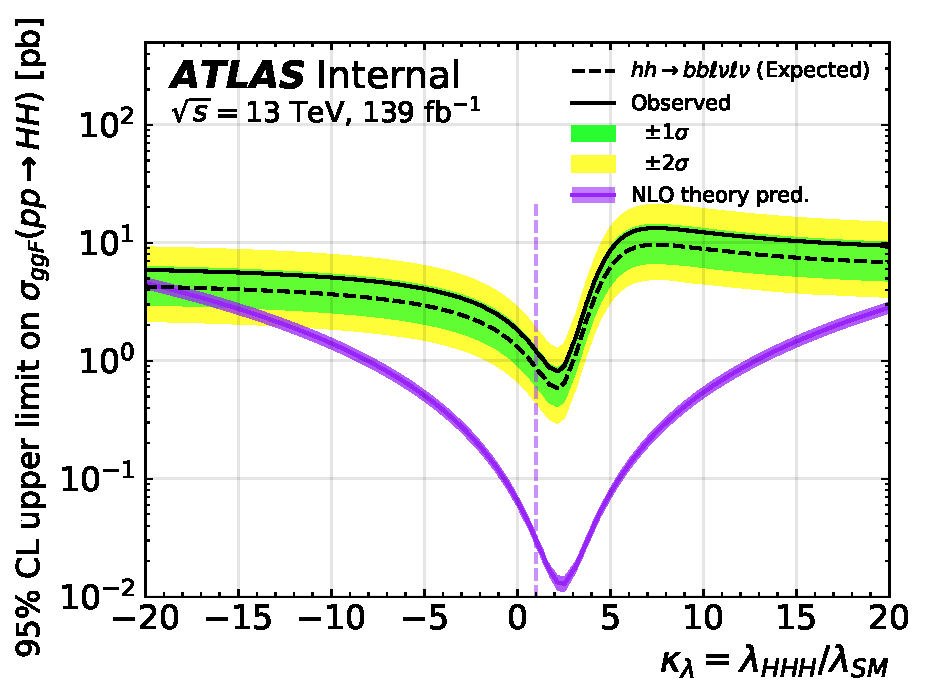
\includegraphics[width=0.6\textwidth]{figures/search_hh/results/wwbb_lambda_scan_may7}
        \caption{
            Expected and observed cross-section upper-limit for the dilepton $hh \rightarrow \bbww$ search
            as a function of the Higgs self-coupling parameter, $\kappa_{\lambda} = \lambda_{hhh} / \lambda_{hhh}^{\text{SM}}$.
            The vertical dashed line indicates the SM scenario with $\kappa_{\lambda} = 1$.
            The $\pm 1\sigma$ and $\pm 2 \sigma$ uncertainty band on the expected upper-limit includes the effects
            of all experimental and modelling systematic uncertainties.
            The NLO theory prediction is taken from Ref.~\cite{deFlorian:2016spz} and described fully
            in Ref.~\cite{HHComb36}.
        }
        \label{fig:hh_lambda_scan}
    \end{center}
\end{figure}

\begin{figure}[!htb]
    \begin{center}
        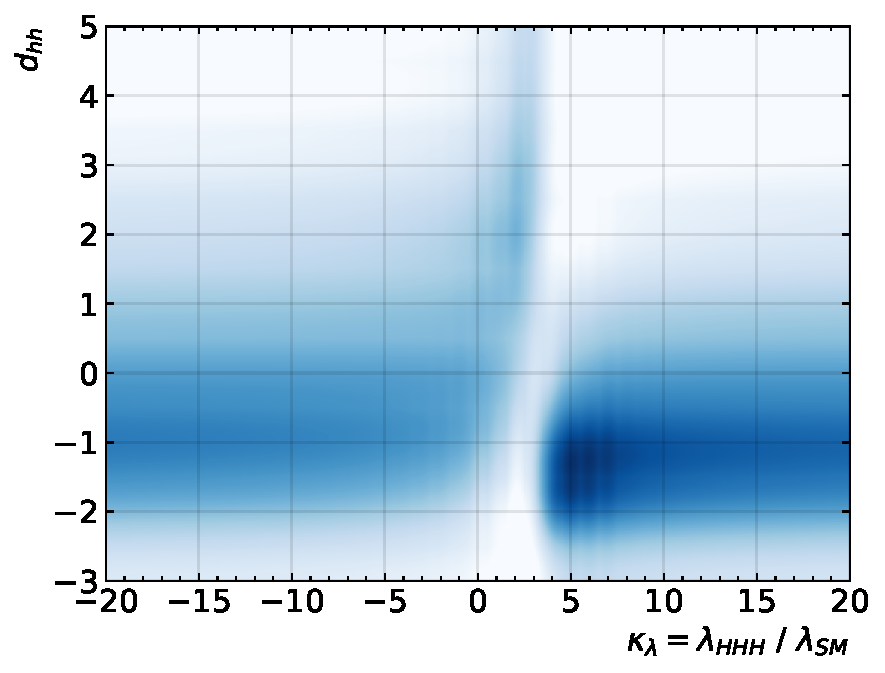
\includegraphics[width=0.6\textwidth]{figures/search_hh/results/dhh_vs_lambda}
        \caption{
            The \dhh distribution as a function of the Higgs self-coupling parameter, $\kappa_{\lambda} = \lambda_{hhh} / \lambda_{hhh}^{\text{SM}}$.
            The trend of the \dhh distribution as a function of $\kappa_{\lambda}$ is directly related to the analysis'
            acceptance to the dilepton $hh \rightarrow \bbww$ signal under non-SM values of $\kappa_{\lambda}$,
            illustrated in Figure~\ref{fig:hh_lambda_scan}.
            The darker the blue color means a higher population of the dilepton $hh \rightarrow \bbww$ signal process.
            The color white indicates that a given region is not populated at all.
        }
        \label{fig:dhh_vs_lambda}
    \end{center}
\end{figure}
